% ============================================================
% FINAL PROJECT REPORT - ENGLISH VERSION
% Project 17: Multimodal Question Answering (VQA)
% Course: CSC15012 - Applications of NLP in Industry
% Student: Le Dinh Minh Quan - 23127460 - 23CNTThuc
% ============================================================
\documentclass[12pt,a4paper]{article}

\usepackage[utf8]{inputenc}
\usepackage{geometry}
\geometry{left=2.3cm, right=2.3cm, top=2.5cm, bottom=2.5cm}
\usepackage{setspace}
\setstretch{1.25}
\usepackage{graphicx}
\usepackage{float}
\usepackage{booktabs}
\usepackage{longtable}
\usepackage{tabularx}
\usepackage{array}
\usepackage{hyperref}
\hypersetup{colorlinks=true, linkcolor=blue, urlcolor=blue, citecolor=blue, breaklinks=true}
\usepackage{xurl}
\usepackage{seqsplit}
\usepackage{listings}
\usepackage{xcolor}
\usepackage{amsmath}
\usepackage{amssymb}
\usepackage{caption}
\usepackage{subcaption}
\usepackage{enumitem}
\usepackage{fancyhdr}
\usepackage{tikz}
\usetikzlibrary{shapes.geometric, arrows.meta, positioning, fit, backgrounds, shadows}

% --- Make long inline code / paths break gracefully ---
\sloppy
\tolerance=2000
\emergencystretch=3em
\hbadness=10000
\setlength{\parskip}{0.15em}

% Helper for breakable monospaced paths
\newcommand{\bpath}[1]{\seqsplit{#1}}
\newcommand{\btt}[1]{\texttt{\seqsplit{#1}}}

% New column type for tabularx: left-aligned and ragged-right with breaking
\newcolumntype{L}{>{\raggedright\arraybackslash}X}

\lstset{
  basicstyle=\ttfamily\small,
  breaklines=true,
  frame=single,
  backgroundcolor=\color{gray!10},
  keywordstyle=\color{blue},
  commentstyle=\color{green!60!black},
  stringstyle=\color{red!70!black},
  showstringspaces=false,
  tabsize=2
}

\pagestyle{fancy}
\fancyhf{}
\fancyhead[L]{\small CSC15012 -- Final Project Report}
\fancyhead[R]{\small Le Dinh Minh Quan -- 23127460}
\fancyfoot[C]{\thepage}

% ============================================================
\begin{document}

% --- TITLE PAGE ---
\begin{titlepage}
\centering
\vspace*{0.5cm}

% HCMUS LOGO: upload logo_hcmus.png to Overleaf to display the logo
\IfFileExists{logo_hcmus.png}{\includegraphics[width=3.5cm]{logo_hcmus.png}\\[0.5cm]}{}

{\large \textbf{VIETNAM NATIONAL UNIVERSITY HO CHI MINH CITY}}\\[0.3cm]
{\Large \textbf{UNIVERSITY OF SCIENCE}}\\[0.3cm]
{\large Faculty of Information Technology}\\[1.5cm]

{\LARGE \textbf{FINAL PROJECT REPORT}}\\[0.5cm]
{\large Course: \textbf{CSC15012 -- Applications of Natural Language\\ Processing in Industry}}\\[1.5cm]

{\Large \textbf{Project 17:}}\\[0.3cm]
{\Large \textbf{Multimodal Question Answering (VQA)}}\\[0.3cm]
{\large A Trainable VQA Core behind a Type-Aware, Abstaining Agent}\\[2cm]

\begin{tabular}{ll}
\textbf{Student:} & Le Dinh Minh Quan \\
\textbf{Student ID:} & 23127460 \\
\textbf{Class:} & 23CNTThuc \\
\end{tabular}

\vfill
{\large Ho Chi Minh City, 2026}
\end{titlepage}

\tableofcontents
\newpage

% ============================================================
\section{Introduction}
% ============================================================

\textbf{Visual Question Answering (VQA)} is the task of answering a free-form natural-language question about the content of an image. Given an \texttt{(image, question)} pair, the system returns a short natural-language answer: a kitchen photo $+$ ``how many chairs are there?'' $\rightarrow$ ``2''; ``what color is the table?'' $\rightarrow$ ``white''; ``is there a stove?'' $\rightarrow$ ``yes''. This is the \textbf{first multimodal-vision project} in the portfolio (P02--P16 reasoned over text, documents, or rendered text); P17 reasons jointly over \textbf{pixels and language}.

This project implements a complete VQA system end-to-end under the package name \texttt{mmqa}, comprising:
\begin{itemize}
  \item A \textbf{trainable VQA core} -- the multimodal transformer \texttt{dandelin/vilt-b32-finetuned-vqa} (ViLT, classification over the canonical 3129-answer VQAv2 vocabulary), fine-tuned. This is the \emph{only} trained artifact.
  \item A deterministic \textbf{agent (D1--D5)} that classifies the question type, runs the model, \textbf{abstains} when the model is uncertain (VQA models are overconfident), and \textbf{constrains} the answer to the question type.
  \item Production-ready serving: a FastAPI REST service, a Gradio UI, Docker, and a one-button Colab H100 autopilot notebook.
  \item An \textbf{offline synthetic-scene harness} (a self-describing scene generator $+$ a torch-free \texttt{SceneStubVQA}) so the whole agent, the official VQA-accuracy scorer, and the tests run with no torch, no model download, and no network.
\end{itemize}

The key design point: the system separates \emph{what is learned} (the VQA model) from \emph{what is engineered} (image decode/resize, tokenization, answer normalization, the question-type classifier, the abstention logic, the type constraint, and scoring -- all pretrained or deterministic).

\textbf{Project Resources (public):}
\begin{itemize}\setlength\itemsep{0.15em}
  \item \textbf{GitHub repository (source code, MIT):} \url{https://github.com/ledinhminhquan/17_Multimodal_QA}
  \item \textbf{Trainable VQA core (HF Hub):} \url{https://huggingface.co/dandelin/vilt-b32-finetuned-vqa} (Apache-2.0)
  \item \textbf{Primary evaluation data (HF Hub):} \url{https://huggingface.co/datasets/lmms-lab/VQAv2} (CC-BY-4.0)
  \item \textbf{Reproducible training:} \texttt{notebooks/MMQA\_Colab\_Training\_H100\_AUTOPILOT.ipynb} with \texttt{notebooks/COLAB\_GUIDE.md}
\end{itemize}

\textbf{Honesty note on results.} The system is fully \emph{deployable} (FastAPI $+$ Gradio $+$ Docker $+$ a one-button Colab H100 autopilot) but is \textbf{not hosted on a public URL}. The verified numbers reported below come from the \textbf{offline synthetic-spine} run: on the synthetic seed scenes the system reaches \emph{model VQA accuracy 1.0} versus a \emph{blind question-only prior of 0.26}, per-type all 1.0, agent coverage 1.0, an automated \textbf{grade of 1.0}, all five decision points fire, and 27 tests pass. The offline accuracy is the \emph{perfect-scene-reading upper bound} (the stub answers from ground truth) -- it validates the \emph{code path}, not real visual reasoning. The honest, publishable accuracy comes from running the same code on the real fine-tuned ViLT over \texttt{lmms-lab/VQAv2} on Colab H100, where the full per-answer-type numbers are produced.

% ============================================================
\section{Business Problem Definition}
% ============================================================

\subsection{Context and Motivation}

The answer in a VQA system is \textbf{grounded in the image}: the same question over two different images should yield two different answers. A system that answers ``yellow'' to ``what color is the banana?'' \emph{without looking at the image} has not solved VQA -- it has merely learned a language prior. Beating that prior is the heart of the problem. VQA is hard for three reasons:
\begin{itemize}
  \item \textbf{Two modalities, one answer}: the model must align image patches with question tokens and fuse them -- harder than image classification or text QA alone.
  \item \textbf{Open-ended questions}: ``how many'', ``what color'', ``is there'', ``where'', ``why'' each imply a different \emph{kind} of answer (a number, a color word, yes/no, a place, a reason).
  \item \textbf{Models are overconfident and prior-driven}: VQA models routinely emit a confident answer that ignores the image. A \emph{calibrated} answer -- including the option to say ``unsure'' -- is as important as raw accuracy.
\end{itemize}

\subsection{Target Users and Stakeholders}

\begin{itemize}
  \item \textbf{Blind and low-vision users} (the canonical VizWiz assistive scenario): photograph surroundings and ask ``what is in front of me?'' / ``is the stove on?''. A wrong-but-confident answer can mislead someone who cannot verify it -- so abstention is a \emph{safety feature}.
  \item \textbf{E-commerce product Q\&A}: ``does this jacket have a hood?'', ``how many are in the pack?'' answered from product imagery.
  \item \textbf{Image search and retrieval}: querying a photo library in natural language.
  \item \textbf{Content-moderation triage}: a fast ``is there X in this image?'' gate where the \emph{abstain / needs-review} path is the right behaviour for ambiguous cases.
  \item \textbf{Developers}: an easy-to-integrate REST API returning answer $+$ confidence $+$ abstain flag.
\end{itemize}

\subsection{Problem Statement}

Given an \texttt{(image, question)} pair, the system must:
\begin{enumerate}
  \item \textbf{Produce a short, type-consistent answer} (a yes/no question gets a yes/no answer; a counting question a number).
  \item \textbf{Abstain honestly} (\texttt{answer="unsure"}, \texttt{needs\_review=true}) when the underlying model is not confident enough, instead of hallucinating.
  \item \textbf{Expose the evidence} (confidence, top-$k$ distribution, and a full D1--D5 decision trace) so a downstream consumer or human reviewer knows when to trust the answer.
\end{enumerate}

\subsection{Why NLP (and Multimodality) is Required}

Questions are open-ended natural language, and the answer space spans yes/no, numbers, colors, objects, and free text. The model must \emph{tokenize and understand} the question and \emph{fuse} it with image features -- a rule-based system cannot map ``how many red squares?'' onto a count of a colour-shape combination in a scene. The agentic value-add (calibrated abstention, type-aware constraint) is itself a language-driven decision over the question type.

\subsection{Success Metrics}

P17 is judged on two axes -- \textbf{accuracy} and \textbf{abstention safety} -- not accuracy alone.

\begin{table}[H]
\centering
\caption{System success metrics}
\begin{tabular}{lll}
\toprule
\textbf{Type} & \textbf{Metric} & \textbf{Target / Reads as} \\
\midrule
Business & Assistive ``unsure'' instead of wrong answer & Abstain when uncertain \\
Business & Coverage / human-review escalation & Route low-confidence to a human \\
Technical & Official VQA soft accuracy (per answer-type) & Beat all four bias baselines \\
Technical & Image-contribution gap (full $-$ blind prior) & Large gap $=$ image is used \\
Technical & Answer-when-confident accuracy vs raw argmax & Higher precision at coverage $<$1 \\
Technical & Re-rank rate (D5 type-constraint activity) & D5 fixes type-wrong argmax \\
\bottomrule
\end{tabular}
\end{table}

A successful P17 is \textbf{accurate when it answers, and quiet when it should be}: the constrained, abstaining agent must beat the raw model on a reliability-adjusted measure.

% ============================================================
\section{Development Infrastructure \& Tooling}
% ============================================================

\subsection{Repository Structure}

The project follows a production-ready Python package structure under \texttt{src/mmqa/}, mirroring the public GitHub repository \url{https://github.com/ledinhminhquan/17_Multimodal_QA} one-to-one. The config, logging, registry, autoreport, monitoring, automation, grading, CLI, and API templates are \emph{reused} from the sibling text projects (P15 \texttt{imgtrans}, P14 \texttt{doctrans}); the \emph{new} vision components are the VQA model wrapper, image handling, the synthetic-scene generator $+$ stub, the official VQA-accuracy metric, the question-type classifier, and the type-aware abstaining agent. Documentation ships \textbf{14 rubric-aligned docs} plus the \texttt{DESIGN\_BRIEF}.

\begin{lstlisting}[basicstyle=\ttfamily\footnotesize]
17_Multimodal_QA/
|-- src/mmqa/
|   |-- config.py  cli.py  logging_utils.py
|   |-- data/        # samples (seed scenes), synth_scene (generator
|   |               #   + answerer), dataset, download
|   |-- models/      # vqa_model (ViLT/BLIP/SceneStub), question_type,
|   |               #   baseline, model_registry
|   |-- vision/      # image_utils (load, read embedded scene,
|   |               #   SceneImage no-PIL carrier)
|   |-- training/    # train_vqa, train_baseline, evaluate, tune,
|   |               #   metrics (VQA accuracy + normalization)
|   |-- agent/       # state, policy (D1-D5), tools, llm_orchestrator,
|   |               #   vqa_agent
|   |-- api/         # schemas, dependencies, main (FastAPI), ui (Gradio),
|   |               #   app_combined
|   |-- analysis/    # error_analysis, latency, per_type
|   |-- autoreport/  # artifact_loader, charts, report_pdf, slides_pptx
|   |-- monitoring/  # drift_report (job-log monitor)
|   |-- automation/  # autopilot (one button)
|   +-- grading/     # checklist (rubric self-check)
|-- configs/  docs/ (14 + DESIGN_BRIEF)  notebooks/  app/  deploy/
|-- sample_data/  scripts/  tests/
|-- Dockerfile  docker-compose.yml  Makefile  pyproject.toml
|-- requirements*.txt  .github/workflows/ci.yml
+-- LICENSE (MIT)  README.md
\end{lstlisting}

\subsection{Technology Stack}

\begin{table}[H]
\centering
\caption{Technology stack}
\small
\begin{tabularx}{\linewidth}{@{} l L @{}}
\toprule
\textbf{Component} & \textbf{Technology} \\
\midrule
Language & Python 3.11 / 3.12 \\
Version Control & Git + GitHub (public repo, MIT) \\
ML Framework & PyTorch + HuggingFace Transformers \\
\textbf{VQA core (trained)} & \texttt{dandelin/vilt-b32-finetuned-vqa} (ViLT, $\sim$113M params; classification head over 3129 answers; Apache-2.0) \\
Custom-vocab base & \texttt{dandelin/vilt-b32-mlm} (Apache-2.0, $\sim$113M) \\
Generative alternative & \texttt{Salesforce/blip-vqa-base} (BSD-3, 384.7M); \texttt{microsoft/git-base-vqav2} (MIT, 177.2M) \\
H100 upgrade & \texttt{Salesforce/blip2-flan-t5-xl} (MIT, $\sim$3.94B); \texttt{Qwen/Qwen2-VL-2B-Instruct} (Apache-2.0) \\
Answer vocab & ViLT config \texttt{id2label} (3129 labels) \\
Processor & \texttt{ViltProcessor} = \texttt{ViltImageProcessor} (RGB, resize $\sim$384px) + \texttt{BertTokenizerFast} \\
Offline harness & synthetic-scene generator + \texttt{SceneStubVQA} (no torch, no network) \\
API & FastAPI + Uvicorn (\texttt{python-multipart} for uploads) \\
UI & Gradio (image upload + question box) \\
Containerization & Docker + Docker Compose (\texttt{libGL} for Pillow) \\
Training GPU & Colab T4 (free floor) $\rightarrow$ A100/L4 (default) $\rightarrow$ H100 (upgrade) \\
Optional LLM brain & \texttt{anthropic} (advisory, OFF by default, never overrides) \\
\bottomrule
\end{tabularx}
\end{table}

\subsection{Training \& Autopilot Workflow}
\label{subsec:workflow}

The end-to-end training-to-deployment workflow is automated by the Colab notebook \texttt{MMQA\_Colab\_Training\_H100\_AUTOPILOT.ipynb}. The user pushes the folder to GitHub (or Drive), opens the notebook, sets the controls in cell 0, and runs \textbf{Runtime $\rightarrow$ Run all}. It fine-tunes the ViLT core (resume-safe), runs the full evaluation, and writes \texttt{report.pdf} $+$ \texttt{slides.pptx} $+$ the submission bundle. The notebook auto-adapts to A100/L4/T4 -- ViLT fine-tunes even on a free T4.

\begin{figure}[H]
\centering
\resizebox{\linewidth}{!}{%
\begin{tikzpicture}[
  node distance=0.32cm,
  step/.style={rectangle, draw=black!60, rounded corners=2pt, thick,
              text width=13.5cm, inner sep=5pt, minimum height=0.75cm,
              align=center, font=\footnotesize},
  setup/.style={step, fill=gray!15},
  train/.style={step, fill=orange!15},
  eval/.style={step, fill=blue!15},
  deploy/.style={step, fill=green!15},
  arrow/.style={-{Stealth[length=2mm]}, thick}
]

\node[setup] (s1) {\textbf{1. Setup (Colab)}: re-verify HF ids + licenses, install deps, pull the 3129-answer vocab from \texttt{dandelin/vilt-b32-finetuned-vqa} config (\texttt{len==3129})};
\node[setup, below=of s1] (s2) {\textbf{2. Synthetic scenes + stub}: \texttt{make\_scene(seed)} self-describing PNGs + \texttt{SceneStubVQA}; assert all five decisions fire offline};
\node[train, below=of s2] (s3) {\textbf{3. Fine-tune ViLT} on \texttt{HuggingFaceM4/VQAv2} train (or zero-shot validate), resume-safe, T4/A100/H100-adaptive (bf16 + LoRA for the upgrade tier)};
\node[eval, below=of s3] (s4) {\textbf{4. Evaluation}: official soft VQA accuracy on \texttt{lmms-lab/VQAv2} validation; overall + per-answer-type + per-question-type};
\node[eval, below=of s4] (s5) {\textbf{5. Baselines}: prior-``yes'', per-type most-common prior, \textbf{blind question-only}, zero-shot ViLT $\rightarrow$ image-contribution gap};
\node[eval, below=of s5] (s6) {\textbf{6. Calibrate D4} (temperature scaling on a held-out split) + abstention/coverage + re-rank rate + risk--coverage curve};
\node[deploy, below=of s6] (s7) {\textbf{7. Auto-gen report \& slides}: \texttt{report\_pdf.py} + \texttt{slides\_pptx.py}};
\node[deploy, below=of s7] (s8) {\textbf{8. Grade + bundle}: \texttt{grading/checklist.py} rubric self-check (verified \textbf{grade 1.0}) + submission bundle};

\foreach \a/\b in {s1/s2, s2/s3, s3/s4, s4/s5, s5/s6, s6/s7, s7/s8}
  \draw[arrow] (\a) -- (\b);

\end{tikzpicture}%
}
\caption{One-button autopilot workflow. The synthetic-scene path (step 2) makes the agent, scorer, and tests runnable with no torch and no network; the real fine-tune (step 3) drops in behind the same \texttt{predict()} contract with no agent changes.}
\label{fig:workflow}
\end{figure}

\paragraph{Key characteristics:}
\begin{itemize}\setlength\itemsep{0.15em}
  \item \textbf{One-button Run-All}: scene generation $+$ fine-tune $+$ evaluation $+$ baselines $+$ calibration $+$ report/slides $+$ grade in one execution.
  \item \textbf{Resume-safe}: the ViLT fine-tune picks up from checkpoints if Colab disconnects.
  \item \textbf{Hardware-adaptive}: auto-detects T4/A100/L4/H100; ViLT ($\sim$113M) fine-tunes comfortably on a free T4 at batch 16--32 @384px; the H100 tier unlocks BLIP-2 / Qwen via bf16 $+$ LoRA.
  \item \textbf{Offline-first}: the synthetic generator $+$ \texttt{SceneStubVQA} guarantee the whole pipeline runs torch-free and network-free in CI; swapping the stub for the real \texttt{ViltForQuestionAnswering} wrapper flips it to production with no agent changes.
  \item \textbf{Self-grading}: \texttt{grading/checklist.py} validates every rubric item after each run (verified grade 1.0).
\end{itemize}

% ============================================================
\section{Data Management}
% ============================================================

\subsection{Data Sources and Roles}

Four data roles are kept strictly separate -- \textbf{TRAIN}, \textbf{EVAL}, \textbf{DEMO/smoke}, and \textbf{OFFLINE/CI} (the synthetic generator) -- plus a fifth pseudo-source: the \textbf{3129-answer vocabulary} from a model config. Every id below was verified on the HuggingFace Hub. \textbf{Any repository that declares no license on the repo is treated as ``license unconfirmed'' and FLAGGED}, even though VQAv2's upstream sources (COCO 2014/2015 images and the VQA annotations) are both CC-BY-4.0.

\begin{table}[H]
\centering
\caption{Data source-of-truth table (licenses verified on HF Hub)}
\small
\setlength{\tabcolsep}{4pt}
\begin{tabularx}{\linewidth}{@{} p{3.6cm} p{2.5cm} L @{}}
\toprule
\textbf{id} & \textbf{Role / License} & \textbf{Schema / notes} \\
\midrule
\texttt{lmms-lab/VQAv2} & PRIMARY EVAL \newline cc-by-4.0 (clean) & 8 cols, clean parquet, embedded PIL images, full 10-annotator \texttt{answers}, \texttt{question\_type}, \texttt{answer\_type}. validation 214.4K (score locally); testdev 107.4K + test 447.8K held out (EvalAI). \textbf{No train split.} \\
\texttt{HuggingFaceM4/VQAv2} & PRIMARY TRAIN \newline \textbf{FLAG} (undeclared) & Only common mirror with a train split ($\sim$443K) + the 10-annotator schema. Loading-script dataset; needs \texttt{trust\_remote\_code=True}; Dataset Viewer 501; may fetch COCO by URL; fragile -- reserve for train only, pin versions. \\
\texttt{Multimodal-Fatima/} \texttt{VQAv2\_sample\_train} & TINY TRAIN, full schema \newline \textbf{FLAG} (undeclared) & 1.0K rows, 13 cols incl. the 10 annotator dicts; works offline once cached; best small set keeping proper soft scoring. \\
\texttt{merve/vqav2-small} & DEMO / smoke \newline \textbf{FLAG} (undeclared) & 3 cols only (\texttt{image}, \texttt{question}, \texttt{multiple\_choice\_answer}), 21.4K val. \textbf{No 10 annotators / no type tags} $\rightarrow$ invalid for official scoring or type routing. Demo only. \\
\texttt{dandelin/vilt-b32-} \texttt{finetuned-vqa} (config) & ANSWER VOCAB \newline apache-2.0 (clean) & A MODEL, not a dataset. Its \texttt{config.json} \texttt{id2label} is the canonical 3129-answer label space (load once; \texttt{len==3129}). \\
\bottomrule
\end{tabularx}
\end{table}

\paragraph{Side / alternative benchmarks (stress tests, not the main loop):} \texttt{lmms-lab/GQA} (MIT, compositional reasoning), \texttt{facebook/textvqa} (CC-BY-4.0, text-in-image -- a side benchmark, \emph{not} the primary task), \texttt{lmms-lab/OK-VQA} (FLAG, knowledge-VQA abstention stress test), \texttt{lmms-lab/VizWiz-VQA} (FLAG; real blind-user photos with an explicit \textbf{unanswerable} label -- the ideal calibrated-abstention test), \texttt{Luo-wj/DAQUAR} (FLAG, indoor scenes).

\paragraph{Explicitly avoided.} \texttt{thangduong0509/daquar\_vqa} -- \textbf{cc-by-nc-sa-4.0 (NON-COMMERCIAL), do not use}; \texttt{jp1924/VisualQuestionAnswering} -- gated + Korean, not VQAv2.

\subsection{The 10-Annotator Structure (why it matters)}

For proper scoring every question carries \textbf{ten human annotator answers}, each a dict \texttt{\{answer, answer\_confidence$\in$\{yes,maybe,no\}, answer\_id$\in$1..10\}}, scored with the official soft VQA accuracy. A dataset without all 10 annotators \emph{cannot} produce this score -- which is exactly why \texttt{merve/vqav2-small} (3 columns) is demo-only. Each question also carries \texttt{answer\_type $\in$ \{yes/no, number, other\}} (the headline 3-bucket breakdown) and a finer \texttt{question\_type} ($\approx$65 buckets).

\subsection{The Synthetic Scene Generator (offline spine)}

The real VQA stack is heavy and flaky (torch $+$ transformers $+$ a vision stack $+$ multi-GB parquet/COCO images, with \texttt{HuggingFaceM4/VQAv2} running a remote loading script). Mirroring P15's OCR \texttt{SeedEngine}, P17 ships a synthetic, self-describing scene generator (\texttt{data/synth\_scene.py}) plus a torch-free \texttt{SceneStubVQA}:
\begin{enumerate}\setlength\itemsep{0.15em}
  \item \texttt{make\_scene(seed)} (PIL only) draws $N$ objects (2--6), each a \texttt{shape $\in$ \{square, circle, triangle\}} and a \texttt{color} from a fixed 6-colour lexicon \texttt{\{red, blue, green, yellow, purple, orange\}}, with non-overlapping bounding boxes on a 224$\times$224 white canvas.
  \item It builds a SCENE SPEC dict (\texttt{objects}, \texttt{counts\_by\_color\_shape}, \texttt{colors\_present}, \texttt{shapes\_present}) and \textbf{embeds it in the PNG} via \texttt{PngImagePlugin.PngInfo().add\_text("scene\_spec", \dots)}, so the image is self-describing and evaluation is fully deterministic.
  \item Templated QA derivation exercises all four routed types -- \texttt{yes\_no}: ``is there a \{shape\}?''; \texttt{count}: ``how many \{color\} \{shape\}s?''; \texttt{color}: ``what color is the \{shape\}?'' (only when that shape is \emph{unique}, so gold is unambiguous); \texttt{object}: ``what shape is the \{color\} object?''. A 10-answer list is synthesized from the gold so the official soft-accuracy code runs unchanged.
  \item \texttt{SceneStubVQA} reads the embedded spec back out, computes the true answer, and returns a \textbf{realistic distribution} ($\approx$0.7--0.9 mass on the truth, the remainder over plausible type-consistent distractors) with a \textbf{difficulty knob} that deliberately lowers \texttt{p\_max} or injects a type-wrong top-1 on a fraction of items, so D4 (abstain) and D5 (re-rank) actually fire and can be unit-tested.
\end{enumerate}
What the synthetic surface proves: the scorer, normalizer, router, abstention gate, and re-rank logic are \emph{correct and wired together}. What it does \emph{not} prove: real-world accuracy -- the stub answers from ground truth, so its ``accuracy'' only reflects the injected difficulty. \textbf{Synthetic accuracy is never quoted as a model result.}

\subsection{Splits, Sizes, and Roles}

\begin{table}[H]
\centering
\caption{Sources, splits, and roles at a glance}
\small
\begin{tabular}{llrcc}
\toprule
\textbf{Source} & \textbf{Split} & \textbf{Size} & \textbf{10 ann.?} & \textbf{Type tags?} \\
\midrule
\texttt{lmms-lab/VQAv2} & validation & 214.4K & yes & yes \\
\texttt{lmms-lab/VQAv2} & testdev/test & 107.4K / 447.8K & held out & held out \\
\texttt{HuggingFaceM4/VQAv2} & train & $\sim$443K & yes & yes \\
\texttt{Multimodal-Fatima/\dots} & train & 1.0K & yes & yes \\
\texttt{merve/vqav2-small} & validation & 21.4K & no & no \\
Synthetic generator & seeded & arbitrary & yes (synth.) & yes \\
ViLT config & --- & 3129 labels & n/a & n/a \\
\bottomrule
\end{tabular}
\end{table}

\paragraph{Default data decision.} TRAIN $=$ \texttt{HuggingFaceM4/VQAv2} (FLAG, \texttt{trust\_remote\_code=True}); EVAL $=$ \texttt{lmms-lab/VQAv2} validation (CC-BY-4.0); DEMO $=$ \texttt{merve/vqav2-small} or \texttt{Multimodal-Fatima/VQAv2\_sample\_train}; VOCAB $=$ ViLT config (3129); CI/OFFLINE $=$ the synthetic generator $+$ \texttt{SceneStubVQA}.

% ============================================================
\section{Model Selection \& Optimization}
% ============================================================

\subsection{Two Answer Regimes}

VQA models split into two families. \textbf{Classification VQA (default)} uses a fixed answer vocabulary (the canonical 3129-answer VQAv2 label space) with a linear head $\rightarrow$ logits $\rightarrow$ softmax $\rightarrow$ top-$k$ answers with clean per-answer probabilities. \textbf{Generative VQA (alternative)} autoregressively decodes free-form answer text (open vocabulary); its confidence is a sequence/token log-probability proxy.

\begin{table}[H]
\centering
\caption{Classification vs generative VQA}
\small
\begin{tabularx}{\linewidth}{@{} l L L @{}}
\toprule
 & \textbf{Classification (DEFAULT)} & \textbf{Generative (alternative)} \\
\midrule
Answer space & Fixed 3129-answer vocab & Open vocabulary (free text) \\
Confidence signal & Clean softmax (\texttt{p\_max}, entropy, margin) & Sequence log-prob (noisier proxy) \\
Default model & \texttt{vilt-b32-finetuned-vqa} ($\sim$113M, Apache-2.0) & \texttt{blip-vqa-base} ($\sim$385M, BSD-3) \\
Evaluation & Direct label lookup $\rightarrow$ clean metric & Decode $+$ normalize $+$ exact-match \\
Ceiling & Gold outside 3129 vocab is \textbf{unreachable} & No fixed-vocab ceiling \\
\bottomrule
\end{tabularx}
\end{table}

\textbf{Why classification is the default.} The softmax over a fixed vocabulary is the \emph{cleanest input for a calibrated abstention gate}: a real probability, a real entropy, and a real top1--top2 margin that the agent thresholds on. Generative models avoid the 3129-answer ceiling but trade away that clean confidence signal -- and the agent is designed against the classification regime.

\subsection{The Default: ViLT Classification}

\textbf{\texttt{dandelin/vilt-b32-finetuned-vqa}} -- Apache-2.0, $\sim$113M params -- is a \emph{single-stream} Vision-and-Language Transformer: image patches and question WordPiece tokens are concatenated and fed through one shared transformer (no heavy object detector), with a classification head over $\sim$3129 answers. It is chosen \emph{because} of the agent, on four criteria in priority order:
\begin{enumerate}\setlength\itemsep{0.1em}
  \item \textbf{Cleanest confidence signal} -- the softmax over 3129 answers is exactly the distribution D3 needs; \texttt{p\_max}, margin, and entropy fall straight out.
  \item \textbf{Type-constrainable output} -- the 3129 vocab already contains \texttt{yes}/\texttt{no}, integers, and colour words, so D5's type-consistency sets are subsets of the model's own classes (re-ranking is a filtered argmax).
  \item \textbf{Permissive license} -- Apache-2.0, the cleanest of any candidate, no flag.
  \item \textbf{Trainable on the floor hardware} -- the smallest core ($\sim$113M) that \emph{fully} fine-tunes on a free-Colab T4 (batch 16--32 @384px).
\end{enumerate}
ViLT is also \emph{already the answer-vocab source}, so the model, the metric buckets, and the agent's constraint sets share one vocabulary by construction. The agent uses the explicit \texttt{ViltProcessor} $+$ \texttt{ViltForQuestionAnswering} path (raw \texttt{outputs.logits} $\rightarrow$ softmax $\rightarrow$ top-$k$) rather than the convenience \texttt{transformers.pipeline}, because it needs the whole distribution, not just argmax.

\subsection{Model Tiers}

\begin{table}[H]
\centering
\caption{Model tier table (ids verified on HF Hub; non-permissive licenses FLAGGED)}
\small
\setlength{\tabcolsep}{4pt}
\begin{tabularx}{\linewidth}{@{} p{4.0cm} p{2.6cm} r L @{}}
\toprule
\textbf{Role / id} & \textbf{License} & \textbf{Params} & \textbf{Class + Processor} \\
\midrule
\textbf{DEFAULT (class.)} \texttt{vilt-b32-finetuned-vqa} & apache-2.0 & $\sim$113M & \texttt{ViltForQuestionAnswering} + \texttt{ViltProcessor} \\
Custom-vocab base \texttt{vilt-b32-mlm} & apache-2.0 & $\sim$113M & \texttt{ViltForQuestionAnswering(num\_labels)} \\
Generative default \texttt{blip-vqa-base} & bsd-3-clause & 384.7M & \texttt{BlipForQuestionAnswering} + \texttt{BlipProcessor} \\
Lightweight gen. \texttt{git-base-vqav2} & mit & 177.2M & \texttt{AutoModelForCausalLM} + \texttt{AutoProcessor} \\
H100 (recommended) \texttt{blip2-flan-t5-xl} & mit & $\sim$3.94B & \texttt{Blip2ForConditionalGeneration} (bf16+LoRA) \\
Clean instr.-VLM \texttt{Qwen2-VL-2B-Instruct} & apache-2.0 & $\sim$2.21B & \texttt{Qwen2VLForConditionalGeneration} (LoRA) \\
\textbf{FLAG} \texttt{llava-1.5-7b-hf} & \textbf{llama2 (NC)} & 7B & upper-bound only, never default \\
\textbf{FLAG} \texttt{Qwen2.5-VL-3B-Instruct} & \textbf{Qwen Research (NC)} & $\sim$3.75B & upper-bound only, never default \\
\bottomrule
\end{tabularx}
\end{table}

\paragraph{AVOID / FLAG.} \texttt{google/pix2struct-vqav2-base} \textbf{does not exist (404)} -- never referenced. \texttt{llava-hf/llava-1.5-7b-hf} (llama2, non-commercial-ish) and \texttt{Qwen/Qwen2.5-VL-3B-Instruct} (Qwen Research, empty HF license) are non-permissive and used only as flagged upper-bound comparisons. (The 7B Qwen2-VL is Apache-clean but $\sim$8B is overkill for a fine-tunable core.)

\subsection{The Baseline Ladder (and the language-prior story)}

VQA's central failure is the \textbf{language prior}: answering from the question text alone (``what color is the banana?'' $\rightarrow$ ``yellow'' regardless of image). The baseline ladder quantifies \emph{how much the image actually helps}; every P17 eval table reports the full model against all of these.

\begin{table}[H]
\centering
\caption{Baseline ladder}
\small
\begin{tabularx}{\linewidth}{@{} c p{3.6cm} L @{}}
\toprule
\textbf{\#} & \textbf{Baseline} & \textbf{Reads as} \\
\midrule
1 & Prior ``yes'' & lower bound for yes/no; near-0 on number/other \\
2 & Most-common-answer (per-type) prior & overall ``yes''; count $\rightarrow$ ``2''; color $\rightarrow$ ``white'' -- the classic prior floor \\
3 & \textbf{Blind / question-only} (no image) & \textbf{measures dataset language bias}; full-model gap over it $=$ the image's contribution \\
4 & Zero-shot pretrained ViLT & calibration point; the bar fine-tuning must beat \\
5 & (optional) image-only ablation & symmetric bias check, blind to the question \\
\bottomrule
\end{tabularx}
\end{table}

Baseline \#3 is load-bearing: \textbf{full-model accuracy $-$ blind-question-only accuracy} is the headline ``does the model use the image'' number. On the offline synthetic spine this gap is \textbf{model 1.0 vs blind prior 0.26}, demonstrating that the system uses the image and not just language priors.

\subsection{The VQA Accuracy Metric}

\textbf{There is NO \texttt{evaluate-metric/vqa} space on the HF Hub} (verified -- returns Not found). The metric is re-implemented from the canonical \texttt{VQAEval} reference. Per-answer credit:
\[
\mathrm{acc}(a) = \min\!\left(1, \frac{\#\{\text{of the 10 annotators whose normalized answer} = a\}}{3}\right)
\]
($\geq$3 matches $\rightarrow$ 1.0; 2 $\rightarrow$ 0.667; 1 $\rightarrow$ 0.333; 0 $\rightarrow$ 0.0). P17 implements the full \textbf{10$\times$ leave-one-out average} (comparing the prediction against 9 annotators at a time) to match the reference exactly, not the \texttt{min(1,matches/3)} simplification -- the two differ when the prediction is itself one of the 10 gold answers. The dataset score is the mean of per-question accuracy $\times$100.

Both the prediction and all 10 gold answers pass through one \textbf{canonical normalization} (single source of truth) -- lowercase; remove punctuation but keep decimals (\texttt{2.5} stays) and merge digit-group commas (\texttt{100,000}$\rightarrow$\texttt{100000}); number-word$\rightarrow$digit; drop articles \texttt{a/an/the}; canonicalize $\sim$80 contractions; collapse spaces. \texttt{evaluate-metric/exact\_match} and \texttt{accuracy} are wired only as auxiliary sanity checks, not the headline soft accuracy.

\subsection{Per-Type Reporting}

A single overall number hides where a VQA model fails. P17 reports two orthogonal breakdowns over the same per-question accuracy values: the headline \textbf{answer-type} 3-bucket breakdown (\texttt{yes/no}, \texttt{number}, \texttt{other}, plus overall, all $\times$100) and the finer \textbf{question-type} ($\approx$65-bucket) appendix table. The typical ordering is \emph{yes/no highest} (a 2-way space, $\sim$80--90\% for a decent model), \emph{other} mid, \emph{number lowest} (counting is the hardest VQA skill).

\subsection{Evaluation Results (Verified Offline; Real Numbers from Colab)}

\begin{table}[H]
\centering
\caption{Verified offline results on the synthetic seed scenes (SceneStubVQA) -- a code-path / plumbing check, NOT a model result}
\begin{tabular}{lc}
\toprule
\textbf{Quantity} & \textbf{Value (offline)} \\
\midrule
Model VQA accuracy (perfect scene reading) & \textbf{1.0} \\
Blind question-only prior & 0.26 \\
Per-type accuracy (yes/no, number, color, object) & all 1.0 \\
Agent coverage & 1.0 \\
Decision points that fire (D1--D5) & all 5 \\
Automated grade (\texttt{grading/checklist.py}) & \textbf{1.0} \\
Unit tests passing & 27 \\
\bottomrule
\end{tabular}
\end{table}

The offline accuracy of 1.0 is the \emph{perfect-scene-reading upper bound}: \texttt{SceneStubVQA} answers from the embedded ground-truth scene spec, so it validates that the scorer, normalizer, router, abstention gate, and re-rank logic are correct and wired together -- a software-correctness guarantee, not a model result. The honest, publishable headline numbers come from running the \emph{same} evaluation code on the real fine-tuned ViLT over \texttt{lmms-lab/VQAv2} validation on Colab H100 (the autopilot, Figure~\ref{fig:workflow}); the expected ordering is yes/no highest, number lowest, reported per answer-type $\times$100 against the four bias baselines. The headline metrics table emitted by every run is shown below.

\begin{table}[H]
\centering
\caption{Headline metrics table (the autoreport template; figures filled on the real Colab H100 run)}
\small
\setlength{\tabcolsep}{4pt}
\begin{tabular}{lcccccc}
\toprule
\textbf{System} & \textbf{Overall} & \textbf{yes/no} & \textbf{number} & \textbf{other} & \textbf{Coverage} & \textbf{Selective acc} \\
\midrule
Prior ``yes'' & --- & --- & --- & --- & 1.00 & --- \\
Most-common (per-type) prior & --- & --- & --- & --- & 1.00 & --- \\
\textbf{BLIND} question-only prior & --- & --- & --- & --- & 1.00 & --- \\
Zero-shot ViLT & --- & --- & --- & --- & 1.00 & --- \\
Fine-tuned ViLT (raw argmax) & --- & --- & --- & --- & 1.00 & n/a \\
\textbf{Fine-tuned ViLT + agent (D4+D5)} & --- & --- & --- & --- & $<$1.00 & --- \\
\bottomrule
\end{tabular}
\end{table}

\subsection{Abstention, Coverage, and Risk--Coverage}

The agent \emph{changes what ``accuracy'' means}: it may abstain instead of guessing, so evaluation separates \emph{did it answer} from \emph{was the answer right}. Let $N$ be total questions and $A$ the answered (non-abstained) subset:
\begin{itemize}\setlength\itemsep{0.1em}
  \item \textbf{Coverage} $= A/N$; \textbf{Abstention rate} $= 1 - A/N$.
  \item \textbf{Answer-when-confident (selective) accuracy} $=$ mean VQA-acc over the $A$ answered items -- how good answers are \emph{when it commits}; should \emph{beat} the raw-argmax model's overall.
  \item \textbf{Full-coverage accuracy} $=$ mean over all $N$ with abstentions scored 0 (apples-to-apples vs an always-answer model).
  \item \textbf{Re-rank rate} $=$ fraction with \texttt{status=ok:reranked}.
\end{itemize}
Because D4's abstention is a calibrated threshold, sweeping it traces a \textbf{risk--coverage curve} (selective accuracy vs coverage); a good gate makes risk fall fast as coverage drops -- the single most defensible artifact in the P17 evaluation.

\subsection{Trade-offs}

\begin{itemize}
  \item \textbf{Accuracy vs vocabulary ceiling}: the classification head is fixed at 3129 answers -- any gold outside is unreachable. The generative regime (BLIP/GIT) avoids the ceiling but trades away the clean softmax confidence the agent relies on.
  \item \textbf{Coverage vs reliability}: the agent declines exactly the cases where the model is overconfident and wrong, trading a little coverage for a large precision gain.
  \item \textbf{Heavy model vs offline testability}: the torch-free \texttt{SceneStubVQA} keeps the agent, scorer, and tests runnable in CI; the real ViLT drops in behind the same \texttt{predict()} contract.
\end{itemize}

% ============================================================
\section{Deployment}
% ============================================================

\subsection{Deployment Formats}

The thing being served is \textbf{not the raw model} -- it is the deterministic agent (\texttt{src/mmqa/agent/}) wrapping the VQA model. Every HTTP and UI response is the agent's output object \texttt{\{answer, status, question\_type, confidence, topk\}}. The system supports \textbf{four} formats:
\begin{enumerate}
  \item \textbf{REST API} (FastAPI): \texttt{GET /healthz}, \texttt{POST /ask}, \texttt{POST /ask-scene}, \texttt{GET /info} (and auto-served \texttt{/docs}, \texttt{/redoc}).
  \item \textbf{Gradio UI}: image upload $+$ question box $+$ confidence bar $+$ abstain/needs-review badge $+$ collapsible top-$k$ table.
  \item \textbf{Docker}: \texttt{Dockerfile} $+$ \texttt{docker-compose.yml} (with \texttt{libGL} baked in for Pillow).
  \item \textbf{Colab H100 autopilot}: one-button fine-tune $+$ eval $+$ report/slides $+$ bundle.
\end{enumerate}
The system is deployable but \textbf{not currently hosted on a public URL}.

\subsection{Serving Architecture}

Both front ends call the \emph{same} \texttt{agent.predict(image, question)} entry point -- there is exactly one inference code path, so the demo and the production endpoint cannot diverge.

\begin{figure}[H]
\centering
\resizebox{\linewidth}{!}{%
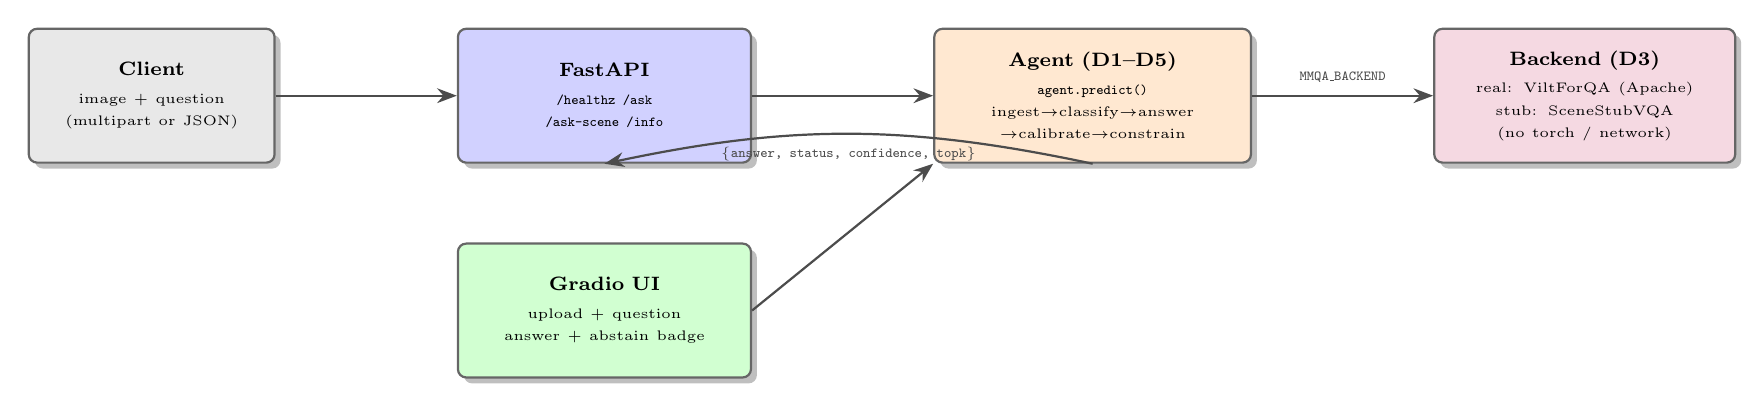
\begin{tikzpicture}[
  node distance=1.0cm and 2.3cm,
  box/.style={rectangle, draw=black!60, rounded corners=3pt, thick,
             text width=3.3cm, minimum height=1.7cm, align=center,
             inner sep=6pt, font=\scriptsize, drop shadow},
  inbox/.style={box, fill=gray!18, text width=2.7cm},
  apibox/.style={box, fill=blue!18},
  uibox/.style={box, fill=green!18},
  agentbox/.style={box, fill=orange!18, text width=3.6cm},
  modelbox/.style={box, fill=purple!15, text width=3.4cm},
  arrow/.style={-{Stealth[length=2.5mm]}, thick, color=black!70}
]

\node[inbox] (user) {%
  \textbf{Client}\\[2pt]
  {\tiny image + question}\\
  {\tiny (multipart or JSON)}
};
\node[apibox, right=of user] (api) {%
  \textbf{FastAPI}\\[2pt]
  {\tiny \texttt{/healthz} \texttt{/ask}}\\
  {\tiny \texttt{/ask-scene} \texttt{/info}}
};
\node[uibox, below=1.0cm of api] (ui) {%
  \textbf{Gradio UI}\\[2pt]
  {\tiny upload + question}\\
  {\tiny answer + abstain badge}
};
\node[agentbox, right=of api] (agent) {%
  \textbf{Agent (D1--D5)}\\[2pt]
  {\tiny \texttt{agent.predict()}}\\
  {\tiny ingest$\rightarrow$classify$\rightarrow$answer}\\
  {\tiny $\rightarrow$calibrate$\rightarrow$constrain}
};
\node[modelbox, right=of agent] (model) {%
  \textbf{Backend (D3)}\\[2pt]
  {\tiny real: ViltForQA (Apache)}\\
  {\tiny stub: SceneStubVQA}\\
  {\tiny (no torch / network)}
};

\draw[arrow] (user) -- (api);
\draw[arrow] (ui.east) -- (agent.south west);
\draw[arrow] (api) -- (agent);
\draw[arrow] (agent) -- node[above=1pt, font=\tiny] {\texttt{MMQA\_BACKEND}} (model);
\draw[arrow] (agent.south) to[bend right=12] node[below=1pt, font=\tiny] {\texttt{\{answer, status, confidence, topk\}}} (api.south);

\end{tikzpicture}%
}
\caption{Serving topology. The API and UI are thin adapters over one \texttt{agent.predict()} path; a single env var (\texttt{MMQA\_BACKEND}) selects the real ViLT backend or the torch-free \texttt{SceneStubVQA}. Swapping the stub for the real wrapper flips the system to production with no agent changes.}
\label{fig:serving}
\end{figure}

\subsection{Endpoints}

\begin{itemize}\setlength\itemsep{0.15em}
  \item \texttt{GET /healthz} -- cheap liveness/readiness probe (no inference); reports backend, \texttt{model\_id}, device, \texttt{model\_loaded}; returns \texttt{503 loading} until the model is ready.
  \item \texttt{POST /ask} -- \texttt{multipart/form-data}: a binary \texttt{image} + a \texttt{question} string (+ optional \texttt{top\_k}). Gated on \texttt{python-multipart}; if missing, \texttt{/ask} returns a clear \texttt{503} while JSON routes stay functional. Returns \texttt{\{answer, status, question\_type, answer\_type, confidence, abstain, needs\_review, topk, model\_id, latency\_ms\}}.
  \item \texttt{POST /ask-scene} -- JSON only (no upload): a \texttt{seed} (server calls \texttt{make\_scene}) or an explicit \texttt{scene\_spec}; identical response schema so clients are interchangeable; powers CI, offline demos, and CPU-only deployments at single-digit-millisecond latency.
  \item \texttt{GET /info} -- registry entry for the active backend: HF id, \textbf{license (with flag)}, params, answer-vocab size (3129), and the D4 thresholds -- so the licensing posture is auditable at runtime.
\end{itemize}

\paragraph{HTTP status mapping.} \texttt{ok}/\texttt{ok:reranked} and both \texttt{abstained:*} statuses return \textbf{200} (abstaining is a valid, successful outcome); \texttt{error:bad\_image}/\texttt{error:bad\_question} return \textbf{422}; \texttt{error:model\_failure} returns \textbf{500}.

\subsection{Docker and GPU vs CPU}

A single image serves both API and UI. The vision stack requires \textbf{\texttt{libGL}} (\texttt{libgl1}) at runtime -- the classic \texttt{libGL.so.1} error on slim images -- so the Dockerfile installs it. Two flavours ship: a small \textbf{CPU/stub image} (\texttt{MMQA\_BACKEND=stub}, Pillow only, no model download, the CI/Space default) and a large \textbf{GPU/real image} (\texttt{MMQA\_BACKEND=vilt}, \texttt{MMQA\_DEVICE=cuda}, torch $+$ transformers). ViLT is small ($\sim$113M) -- a T4 serves it with low latency; no A100/H100 is needed to \emph{serve} (those tiers are for training / the heavier generative upgrades). The agent never assumes a GPU: if CUDA is requested but unavailable it logs a warning and falls back to CPU.

\subsection{Configuration}

All deployment knobs are env vars read by the reused config object. Key ones: \texttt{MMQA\_BACKEND} (\texttt{stub}/\texttt{vilt}), \texttt{MMQA\_MODEL\_ID}, \texttt{MMQA\_DEVICE}, \texttt{MMQA\_TOP\_K} (5), the D4 thresholds \texttt{MMQA\_TAU\_CONF} (0.30) / \texttt{MMQA\_TAU\_ENT} (1.5) / \texttt{MMQA\_TAU\_MARGIN} (0.10), \texttt{MMQA\_TEMPERATURE} (1.0, tuned on a held-out split), \texttt{MMQA\_MAX\_IMAGE\_MB} (10), \texttt{MMQA\_RETAIN\_IMAGES} (\texttt{false}, privacy default), and \texttt{MMQA\_ENABLE\_LLM} (\texttt{false}; \texttt{ANTHROPIC\_API\_KEY} read only when enabled). The abstention gate is a \emph{tuned} gate, not a hard-coded constant, because VQA models are overconfident.

% ============================================================
\section{Agentic AI Component}
% ============================================================

\subsection{Why an Agent at All}

A stock ViLT/BLIP model does exactly one thing: raw \textbf{argmax}. That is not enough for production -- VQA classifiers are notoriously overconfident, the argmax is frequently \emph{fluent but type-wrong} (``cat'' to ``how many?''), and a bare model cannot say ``I don't know.'' The P17 agent is a deterministic \textbf{finite-state machine} \texttt{ingest $\rightarrow$ classify $\rightarrow$ answer $\rightarrow$ calibrate $\rightarrow$ constrain} with \textbf{five decision points}; only D3 touches the model, the other four are pure deterministic logic over the model's own top-$k$ distribution and the question text. With \textbf{zero extra training} it adds two production behaviours: \textbf{calibrated abstention} (says ``unsure'' instead of guessing) and a \textbf{type-aware answer constraint $+$ re-rank}.

\begin{figure}[H]
\centering
\resizebox{0.92\linewidth}{!}{%
\begin{tikzpicture}[
  node distance=0.3cm,
  step/.style={rectangle, draw=black!60, rounded corners=2pt, thick,
              text width=13.0cm, inner sep=5pt, minimum height=0.7cm,
              align=center, font=\footnotesize},
  gate/.style={step, fill=gray!15},
  route/.style={step, fill=blue!12},
  model/.style={step, fill=purple!15},
  decide/.style={step, fill=red!12},
  cons/.style={step, fill=green!15},
  arrow/.style={-{Stealth[length=2mm]}, thick}
]

\node[gate] (d1) {\textbf{D1 INGEST} (input gate, PIL + regex, no torch): valid nonzero RGB image (var $>$ eps) AND non-empty interrogative question ($\geq$1 alpha token, len 1--128) \quad$\rightarrow$\quad else HALT \texttt{error:bad\_image} / \texttt{error:bad\_question}};
\node[route, below=of d1] (d2) {\textbf{D2 CLASSIFY} (question-type router, first-match-wins): \texttt{is/are/does..}$\rightarrow$\texttt{yes\_no}\{yes,no\} \;|\; \texttt{how many}$\rightarrow$\texttt{count}\{0..20,none\} \;|\; \texttt{what color}$\rightarrow$\texttt{color}\{lexicon\} \;|\; else \texttt{object/other} (open)};
\node[model, below=of d2] (d3) {\textbf{D3 ANSWER} (the ONLY model call): real \texttt{ViltForQuestionAnswering}$\rightarrow$logits | offline \texttt{SceneStubVQA} \quad$\rightarrow$\quad \texttt{topk}(k=5), \texttt{p\_max}, margin, entropy, regime \quad(exception$\rightarrow$HALT \texttt{error:model\_failure})};
\node[decide, below=of d3] (d4) {\textbf{D4 CALIBRATE} (calibrated abstention): \texttt{p\_max}$\geq\tau_{\text{conf}}$ AND margin$\geq\tau_{\text{margin}}$ AND entropy$\leq\tau_{\text{ent}}$ (temperature-scaled, per-type) \quad$\rightarrow$\quad else \texttt{answer="unsure"} \texttt{abstained:low\_confidence} (+\texttt{needs\_review})};
\node[cons, below=of d4] (d5) {\textbf{D5 CONSTRAIN} (type-consistency + re-rank within top-$k$): \texttt{topk[0]} in allowed set$\rightarrow$\texttt{ok} | a lower top-$k$ entry consistent$\rightarrow$\texttt{ok:reranked} | none matches$\rightarrow$\texttt{abstained:type\_mismatch}};

\foreach \a/\b in {d1/d2, d2/d3, d3/d4, d4/d5}
  \draw[arrow] (\a) -- (\b);

\end{tikzpicture}%
}
\caption{The deterministic 5-decision agent FSM. It is strictly forward (no loops); every path reaches a terminal \texttt{ok*}/\texttt{abstained:*} state or short-circuits to an \texttt{error:*} halt. The final output is \texttt{\{answer, status, question\_type, answer\_type, confidence, topk, needs\_review, trace\}}.}
\label{fig:agent}
\end{figure}

\subsection{The Five Decision Points}

\begin{table}[H]
\centering
\caption{Consolidated decision table}
\small
\setlength{\tabcolsep}{4pt}
\begin{tabularx}{\linewidth}{@{} c p{1.6cm} L L @{}}
\toprule
\textbf{D} & \textbf{Stage} & \textbf{Gates on (signal)} & \textbf{Branches} \\
\midrule
D1 & Ingest & valid RGB image (var $>$ eps) AND non-empty interrogative question ($\leq$128 tok) & $\rightarrow$ D2 \;|\; \texttt{error:bad\_image} / \texttt{error:bad\_question} (HALT, no model call) \\
D2 & Classify & leading-keyword question type, first-match-wins (\texttt{how many} beats \texttt{how}; \texttt{what color} beats \texttt{what}) & always routes to \texttt{\{yes\_no, count, color, object/other\}}; the bucket defines the allowed set for D5 \\
D3 & Answer & model \texttt{predict()} $\rightarrow$ \texttt{topk}, \texttt{p\_max}, margin, entropy, regime (the only model call) & $\rightarrow$ D4 with distribution \;|\; \texttt{error:model\_failure} (HALT) \\
D4 & Calibrate & \texttt{p\_max}$\geq\tau_{\text{conf}}$ AND margin$\geq\tau_{\text{margin}}$ AND entropy$\leq\tau_{\text{ent}}$ (temperature-scaled) & confident $\rightarrow$ D5 \;|\; any fails $\rightarrow$ \texttt{abstained:low\_confidence} $\rightarrow$ ``unsure'' \\
D5 & Constrain & \texttt{topk[i]} $\in$ allowed set for the D2 type (re-rank within top-$k$) & \texttt{ok} / \texttt{ok:reranked} \;|\; no match $\rightarrow$ \texttt{abstained:type\_mismatch} $\rightarrow$ ``unsure'' \\
\bottomrule
\end{tabularx}
\end{table}

D4 requires \textbf{three} signals to agree (a single signal is unreliable on overconfident models): max probability \texttt{p\_max} vs \texttt{tau\_conf} (0.30; per-type yes\_no 0.40, count 0.45), top1--top2 margin vs \texttt{tau\_margin} (0.10), and Shannon entropy $H=-\sum p_i \ln p_i$ vs \texttt{tau\_entropy} (1.50 nats), all measured on the \emph{temperature-scaled} distribution. D5 re-ranks within the top-$k$ but never invents an answer outside the model's own candidates. Every decision appends one structured, reason-bearing entry to a \texttt{ToolTrace} audit log; the trace is deterministic and replayable, and CI asserts on the trace, not just the final answer.

\paragraph{Optional LLM brain (advisory, OFF by default).} An optional \texttt{anthropic} ``brain'' is consulted only in ambiguous cases and is wired so it \textbf{can never override the deterministic gates} -- it cannot introduce an answer outside the top-$k$, relax a threshold, or turn an abstention into an assertion. With it disabled (the default), the agent is fully deterministic, offline, and reproducible -- the configuration used for all CI, grading, and the headline metrics.

\subsection{Example Decision Traces}

\begin{lstlisting}
# Example A -- clean count, re-ranked to type (scene: 3 red squares, 1 blue circle)
Input: "how many red squares?"
  D1 accept : image var > eps; interrogative, 4 tokens
  D2 route  : leading "how many" -> count ; allowed = {0..20, none}
  D3 predict: topk=[("squares",0.41),("3",0.33),("2",0.14),("4",0.08),("red",0.04)]
              p_max=0.41, margin=0.08, entropy=1.39
  D4 confident: temperature calibration lifts p_max->0.47 (>=0.45),
                margin 0.12 >= 0.10, entropy 1.39 <= 1.50  -> CONFIDENT
  D5 re-rank : topk[0]="squares" not in count_lexicon; scan finds "3" -> promote
Output: {answer:"3", status:"ok:reranked", question_type:"count",
         answer_type:"number", confidence:0.47, needs_review:false}
         # correct, where raw argmax ("squares") would have scored 0

# Example B -- low confidence, abstain (blurry scene, two triangles, ambiguous)
Input: "what color is the triangle?"
  D1 accept : valid image + interrogative question
  D2 route  : "what color" -> color ; allowed = color_lexicon
  D3 predict: topk=[("red",0.28),("orange",0.24),("blue",0.20),("green",0.16),("purple",0.12)]
              p_max=0.28, margin=0.04, entropy=1.59
  D4 abstain: p_max 0.28 < 0.30 ; margin 0.04 < 0.10 ; entropy 1.59 > 1.50 (fails all 3)
Output: {answer:"unsure", status:"abstained:low_confidence", question_type:"color",
         confidence:0.28, needs_review:true}   # refused rather than guessing "red"

# Example C -- bad input, hard halt (all-white image)
Input: image (all white) + "how many cats?"
  D1 reject : pixel variance 3e-6 < blank_pixel_var_eps 1e-4 -> degenerate-blank
Output: {status:"error:bad_image", trace:[D1]}  # model never called; no image retained
\end{lstlisting}

\subsection{Value-Add Over Raw Argmax}

The agent adds two production behaviours with no extra training, both from deterministic logic over the model's own top-$k$ $+$ softmax: (1) \textbf{calibrated abstention (D4)} -- the system refuses to answer when uncertain instead of emitting a confident wrong answer (headline metric: answer-when-confident accuracy and abstention rate vs raw argmax); and (2) \textbf{type-aware constraint $+$ re-rank (D2$\rightarrow$D5)} -- the same frozen model yields higher \emph{constrained} accuracy. Because the five decision points are explicit and traced, the orchestration is auditable and offline-testable -- the whole FSM runs against \texttt{SceneStubVQA} with no torch and no network.

% ============================================================
\section{Continual Learning \& Monitoring}
% ============================================================

\subsection{What the Deployed System Emits}

Every \texttt{agent.predict()} call already produces a structured, auditable record (the agent's value-add \emph{is} its instrumentation); monitoring aggregates these over time with no new instrumentation. One JSON line per request logs: \texttt{request\_id}/\texttt{ts}; \texttt{question\_type}/\texttt{answer\_type}; \texttt{topk}; \texttt{p\_max}/margin/entropy; \texttt{status}; \texttt{answer}; re-rank fields; per-stage \texttt{latency\_ms}; and \texttt{model\_sha}/\texttt{vocab\_sha}/\texttt{agent\_cfg\_sha} for version attribution. \textbf{No raw image bytes and no raw user question are persisted by default}; only a small \texttt{image\_meta} block of derived scalars (dimensions, pixel variance, blur estimate) is kept -- enough for image-domain drift, nothing reconstructable.

\subsection{Monitoring Strategy}

\texttt{monitoring/drift\_report.py} consumes a window of job logs (plus an optional labeled slice) and emits one report. Four signal families are tracked:
\begin{itemize}\setlength\itemsep{0.15em}
  \item \textbf{Operational (label-free, 100\% of traffic)}: coverage, abstention rate split by cause (\texttt{low\_confidence} vs \texttt{type\_mismatch}), error rate, re-rank rate, and per-stage latency (p50/p95/p99). A rising low-confidence abstention rate is the earliest label-free signal of input or calibration drift -- all tracked \emph{per question\_type} (count is harder).
  \item \textbf{Confidence-signal drift (label-free)}: PSI / 1-D Wasserstein on the \texttt{p\_max}/margin/entropy distributions vs a frozen reference window -- a direct precursor to a calibration problem.
  \item \textbf{Accuracy on a labeled slice}: the same official VQA-accuracy metric (overall $+$ per-answer-type $+$ per-question-type), \textbf{answer-when-confident accuracy @ coverage}, and the baselines re-scored on the slice -- crucially the \textbf{blind/question-only} prior, since a shrinking full-model-minus-blind gap is a flashing red light that the model has reverted to the language shortcut.
  \item \textbf{Distribution drift}: answer-distribution (mode-collapse onto priors, vocab-edge pressure), question-distribution (\texttt{question\_type} mix, router fall-through rate), and image-domain drift (resolution/aspect/\texttt{pixel\_var}/blur on derived scalars only; optional consented-only CLIP-embedding drift).
\end{itemize}

\subsection{The Answer-Vocabulary Growth Problem (P17-specific)}

The classification head is fixed at 3129 answers -- any gold outside is unreachable, and over time real questions drift toward answers the head cannot emit. Vocab pressure is tracked via the \textbf{unreachable-gold rate}, \texttt{other}-bucket mass and \texttt{type\_mismatch} abstentions on closed-type (color/count) questions, and out-of-vocab top-$k$ saturation -- all using the \emph{same} normalization as the metric so a ``new'' answer is genuinely new.

\subsection{Continual Learning -- Triggers and Response Ladder}

A trigger does not mean ``retrain immediately'' -- it means ``run the response ladder,'' escalating only as far as needed (cheapest fix first):
\begin{enumerate}\setlength\itemsep{0.15em}
  \item \textbf{Recalibrate (config only)}: re-fit temperature $T$ and re-tune \texttt{tau\_conf}/\texttt{tau\_ent}/\texttt{tau\_margin} per question\_type on a fresh slice -- no training; most coverage/accuracy regressions are fixed here.
  \item \textbf{Update deterministic logic}: extend the keyword classifier / D5 lexicons when router fall-through rises -- no training.
  \item \textbf{Vocabulary refresh $+$ re-fine-tune}: expand the head from \texttt{dandelin/vilt-b32-mlm}; the metric, D5 constraint sets, and report buckets must all use the new vocab and \texttt{vocab\_sha}.
  \item \textbf{Full re-fine-tune of the core}: on a sustained labeled-slice accuracy drop recalibration cannot fix, or a closing blind-prior gap.
\end{enumerate}
Triggers are AND-gated against volume (must persist over N windows) and per-slice. \textbf{Feedback capture} (thumbs up/down; human corrections of \texttt{abstained:*} items -- the highest-value training signal) feeds the labeled slice and the production-derived training set, normalized into the VQAv2 10-annotator schema, deduped, and quality-reviewed before training. Promotion is staged \textbf{shadow $\rightarrow$ canary $\rightarrow$ promote}, gated on: no regression on yes/no, improved/held answer-when-confident accuracy @ matched coverage, a maintained-or-widened blind-prior gap, maintained/improved ECE, and a passing offline \texttt{SceneStubVQA} regression. Rollback is a \texttt{model\_sha} switch since the agent contract is version-independent. Every box in this loop is exercisable with no torch and no network via the synthetic generator $+$ stub.

% ============================================================
\section{Data Privacy \& Model Robustness}
% ============================================================

\subsection{Privacy}

P17 is the first project whose \emph{input is a user photograph}, which can contain faces, homes, screens, documents, medical images, and location cues -- and the assistive (VizWiz) use case is exactly the population least able to vet what is uploaded. P17 adopts a \textbf{minimise, localise, do-not-retain} posture:
\begin{itemize}\setlength\itemsep{0.15em}
  \item \textbf{Local / on-device processing by default}: the small permissive core (ViLT $\sim$113M Apache; BLIP-base $\sim$385M) runs self-hosted -- no image need leave the deployment boundary.
  \item \textbf{No raw-image retention by default} (\texttt{retain\_images=False}): \texttt{POST /ask} processes bytes in memory and discards them; nothing is written to disk or logs.
  \item \textbf{The LLM brain is OFF by default}, advisory-only; with it off no image or question is sent to any external provider.
  \item \textbf{Logs carry derived signals, not pixels}; question logging is opt-in (a question can itself be sensitive, e.g.\ ``is this mole cancerous?'').
  \item \textbf{EXIF/GPS stripped}: only the decoded RGB array is used (note the asymmetry -- the synthetic generator deliberately embeds \texttt{scene\_spec} in PNG metadata for test fixtures \emph{only}, never on real uploads).
  \item P17 \emph{does not} do face recognition, identity inference, or demographic classification.
\end{itemize}

\subsection{Robustness -- Failure Modes and Mitigations}

\begin{table}[H]
\centering
\caption{Failure-mode $\rightarrow$ mitigation summary (most live in the deterministic agent and are offline-testable)}
\small
\setlength{\tabcolsep}{4pt}
\begin{tabularx}{\linewidth}{@{} L L c c @{}}
\toprule
\textbf{Failure mode} & \textbf{Primary mitigation} & \textbf{Where} & \textbf{Offline-test} \\
\midrule
Model overconfidence & Calibrated abstention (\texttt{p\_max}+entropy+margin, temperature-scaled, per-type) & D4 & Yes \\
Language-prior shortcut & Blind question-only baseline + per-type accuracy + image-dependent gates & Eval + D4/D5 & Yes \\
Out-of-vocab answers & 3129-vocab ceiling documented/reported; generative escape hatch (BLIP/GIT) & Metric + model & Partial \\
Unanswerable questions & Abstain (flat/low-margin $\rightarrow$ ``unsure''); VizWiz \texttt{unanswerable} eval & D4 & Yes \\
Image blur / corrupt / blank & Input gate: RGB-decode + pixel-variance check & D1 & Yes \\
Empty / non-question text & Input gate: interrogative + length + alpha-token checks & D1 & Yes \\
Adversarial / leading / type-wrong & Type-consistency gate + top-$k$ re-rank, else abstain & D5 (+D4) & Yes \\
Demographic / dataset bias & Measure (blind baseline, per-type), assist-not-assert, clean-license data & Eval + ethics & Partial \\
Heavy / flaky deps & Torch-free \texttt{SceneStubVQA} + synthetic scenes; availability-gated real path & harness & Yes \\
\bottomrule
\end{tabularx}
\end{table}

The two halves are linked: the same agent gates that protect reliability (D4 abstention, D5 type-consistency) are what keep the system from asserting confident, wrong, potentially harmful answers about someone's medicine or surroundings. Because the synthetic harness runs torch-free, this privacy-and-robustness behaviour is verified in CI on every run.

% ============================================================
\section{Project Management}
% ============================================================

This project was completed \textit{individually}. The plan spans eight weeks of part-time effort organised into nine milestones (M0--M8); the critical path is \texttt{M1 (scenes+stub) $\rightarrow$ M3 (metric) / M4 (qtype) $\rightarrow$ M5 (agent) $\rightarrow$ M6 (eval \& baselines)}, with the real fine-tune (M2) deliberately \emph{off} the offline critical path.

\begin{table}[H]
\centering
\caption{Project timeline (nine milestones)}
\small
\begin{tabularx}{\linewidth}{@{} l l L @{}}
\toprule
\textbf{M\#} & \textbf{Week(s)} & \textbf{Milestone / exit criterion} \\
\midrule
M0 & 1 & Research \& scaffold: re-verify HF ids + licenses (confirm \texttt{pix2struct-vqav2-base} 404), pull the 3129 vocab (\texttt{len==3129}) \\
M1 & 1--2 & Synthetic scenes + stub: hash-stable PNGs, all 5 decisions fire, soft-VQA scorer torch-free \\
M2 & 2--3 & VQA wrapper + fine-tune: uniform \texttt{predict()}; ViLT zero-shot beats bias baselines (parallel, off critical path) \\
M3 & 3--4 & VQA-accuracy metric: re-implemented \texttt{VQAEval} (normalization + 10$\times$ LOO + per-type) \\
M4 & 4 & Question-type classifier: 10-rule keyword scheme, order-critical, $\rightarrow$ 4 buckets \\
M5 & 5--6 & Agentic FSM: D1--D5 + temperature scaling + per-decision trace + advisory brain OFF \\
M6 & 6 & Evaluation \& baselines: soft VQA acc + 4 baselines + answer-when-confident/coverage/re-rank \\
M7 & 7 & Deploy: FastAPI (\texttt{/ask}, \texttt{/ask-scene}) + Gradio + Docker (libGL) + HF Space \\
M8 & 8 & Hardening \& docs: robustness suite, ethics/privacy, monitoring/grading, final report \\
\bottomrule
\end{tabularx}
\end{table}

\textbf{Risk register (top items).} R1 overconfident models $\rightarrow$ tuned multi-signal D4 gate; R2 language-prior bias $\rightarrow$ mandatory blind baseline; R3 \texttt{HuggingFaceM4/VQAv2} fragility $\rightarrow$ reserve for train only, pin versions; R4 3129-vocab ceiling $\rightarrow$ one shared vocab, report OOV rate; R5 non-commercial/undeclared licenses $\rightarrow$ ship only declared-permissive; R6 stub too easy $\rightarrow$ realistic distribution + difficulty knob; R7 metric re-implementation bugs $\rightarrow$ unit-test decimals/commas/articles/contractions. \textbf{Scaling reflection}: in a team setting the workstreams (data/vision, VQA core, metric, agent, deploy, docs) would parallelize behind the same \texttt{predict()} contract.

% ============================================================
\section{Ethics \& Responsible AI}
% ============================================================

\subsection{Who Benefits, Who Could Be Harmed}

Beneficiaries: blind/low-vision users (assistive scene Q\&A), shoppers (product Q\&A), and anyone querying photo libraries. Potential harms concentrate in high-stakes use: a confident-looking wrong answer delivered to someone who \emph{cannot verify it} (the accessibility user), or to a medical/safety/legal image where a COCO-scene model is out of its competence domain but still answers.

\subsection{Assist and Abstain, Never Assert Certainty}

P17's guiding principle is enforced by the \textbf{D4 calibrated abstention gate}: the tool assists; it never asserts certainty. When the model is not confident enough the system returns \texttt{answer="unsure"} with \texttt{needs\_review=true} instead of a guess. Beyond low-confidence abstention, \textbf{medical, diagnostic, dosage, legal, and safety-critical questions are treated as out of scope}, and the deployment surface states plainly: \emph{``P17 answers everyday questions about ordinary scenes. It is not a medical, diagnostic, legal, or safety device.''} The headline reliability metric -- answer-when-confident accuracy plus abstention rate vs raw argmax -- explicitly measures the precision/coverage trade abstention buys.

\subsection{Bias: Surfaced, Not Hidden}

P17 does not claim to eliminate the language prior -- it \textbf{measures and publishes} it. The mandatory \textbf{blind / question-only baseline} (and the gap to it) is reported every run as the honest measure of how much the image contributes; on the offline spine the gap is \textbf{1.0 vs 0.26}. Per-answer-type and per-question-type accuracy are always broken out so a strong aggregate cannot mask weak counting or open-vocab performance. The training images are COCO 2014/2015 scenes -- a geographically and culturally skewed collection -- so the model inherits demographic bias; P17 therefore \textbf{does not infer protected attributes} of people in images, and discloses the fixed 3129-answer vocabulary ceiling so ``not in vocab'' is not mistaken for ``not true.''

\subsection{Transparency, License Hygiene, and Human-in-the-Loop}

Every answer ships with its calibrated confidence, the top-$k$ distribution, and the full auditable D1--D5 trace -- legible, not oracular. License hygiene is honoured: ship only declared-permissive assets (ViLT Apache-2.0, BLIP BSD-3, GIT/BLIP-2 MIT; \texttt{lmms-lab/VQAv2} CC-BY-4.0, \texttt{lmms-lab/GQA} MIT); FLAG every undeclared mirror; \textbf{never} ship the non-commercial \texttt{llava-1.5-7b-hf} (llama2) or \texttt{Qwen2.5-VL-3B} (Qwen Research) as the default core, and never use \texttt{thangduong0509/daquar\_vqa} (CC-BY-NC-SA). Uncertainty \textbf{routes to a person}: every \texttt{abstained:*} item is flagged for human review rather than answered, the trace makes review tractable, and the optional LLM brain is advisory-only and never overrides the safety logic.

\subsection{Guiding Principle}

\begin{quote}
A VQA system that admits ``I'm not sure'' is more trustworthy than one that is always confident and sometimes wrong -- especially for the people who cannot check its answer for themselves.
\end{quote}

% ============================================================
\section{Conclusion \& Future Work}
% ============================================================

\subsection{Summary}

\begin{itemize}\setlength\itemsep{0.15em}
  \item A complete end-to-end VQA system (\texttt{mmqa}): a \textbf{trainable ViLT core} (Apache-2.0, classification over 3129 answers) wrapped by a deterministic \textbf{5-decision agent} (input gate, type router, model, calibrated abstention, type-consistency re-rank).
  \item The official soft VQA accuracy is re-implemented from \texttt{VQAEval} (no HF metric exists), with the 10$\times$ leave-one-out average, one canonical normalizer, and per-answer-type / per-question-type reporting against a four-rung bias-baseline ladder.
  \item \textbf{Verified offline (synthetic spine)}: model accuracy 1.0 vs blind prior 0.26, per-type all 1.0, coverage 1.0, all 5 decisions fire, automated grade 1.0, 27 tests pass -- a software-correctness guarantee; the honest publishable numbers come from the real ViLT on \texttt{lmms-lab/VQAv2} via the Colab H100 autopilot.
  \item \textbf{Deployable} four ways (FastAPI, Gradio, Docker, Colab autopilot) over one \texttt{agent.predict()} path; the torch-free \texttt{SceneStubVQA} flips to the real model behind the same \texttt{predict()} contract with no agent changes.
  \item \textbf{Responsible by design}: no raw-image retention by default, LLM brain off, abstain-never-assert, blind-baseline bias reporting, and FLAGged license hygiene.
\end{itemize}

\subsection{Future Work}

\begin{enumerate}\setlength\itemsep{0.15em}
  \item \textbf{Real-VQAv2 headline numbers}: complete the Colab H100 fine-tune and publish overall $+$ per-answer-type accuracy with the risk--coverage curve.
  \item \textbf{Generative escape hatch}: switch the core to \texttt{Salesforce/blip-vqa-base} (BSD-3) to lift the 3129-vocab ceiling for open-ended traffic, documenting the noisier logprob confidence.
  \item \textbf{H100 upgrade}: \texttt{Salesforce/blip2-flan-t5-xl} (MIT) via bf16 $+$ LoRA for clean constrained/instruction decoding that fits the agent's type constraints.
  \item \textbf{Calibration depth}: reliability diagrams + ECE before/after temperature scaling, and per-question-type thresholds.
  \item \textbf{Abstention external validity}: evaluate the gate on \texttt{lmms-lab/VizWiz-VQA}'s explicit \texttt{unanswerable} label (abstain-vs-unanswerable agreement).
  \item \textbf{Live demo}: publish a Gradio HF Space (stub default on CPU; clean Apache ViLT on a T4).
\end{enumerate}

% ============================================================
\newpage
\begin{thebibliography}{9}

\bibitem{vilt} Kim, W., Son, B., \& Kim, I. (2021). ViLT: Vision-and-Language Transformer Without Convolution or Region Supervision. \textit{ICML 2021}.

\bibitem{vqa} Antol, S., et al. (2015). VQA: Visual Question Answering. \textit{ICCV 2015}.

\bibitem{vqav2} Goyal, Y., Khot, T., Summers-Stay, D., Batra, D., \& Parikh, D. (2017). Making the V in VQA Matter: Elevating the Role of Image Understanding in Visual Question Answering. \textit{CVPR 2017}.

\bibitem{blip} Li, J., Li, D., Xiong, C., \& Hoi, S. (2022). BLIP: Bootstrapping Language-Image Pre-training. \textit{ICML 2022}.

\bibitem{coco} Lin, T.-Y., et al. (2014). Microsoft COCO: Common Objects in Context. \textit{ECCV 2014}.

\bibitem{vizwiz} Gurari, D., et al. (2018). VizWiz Grand Challenge: Answering Visual Questions from Blind People. \textit{CVPR 2018}.

\bibitem{transformers} Wolf, T., et al. (2020). Transformers: State-of-the-Art Natural Language Processing. \textit{EMNLP 2020}.

\bibitem{fastapi} Ram\'irez, S. (2018). FastAPI. \url{https://fastapi.tiangolo.com/}

\bibitem{guo} Guo, C., Pleiss, G., Sun, Y., \& Weinberger, K.~Q. (2017). On Calibration of Modern Neural Networks. \textit{ICML 2017}. (Temperature scaling.)

\end{thebibliography}

\end{document}
